\documentclass{report}
\usepackage[english]{babel}
\usepackage{microtype}
\usepackage{amsmath,amssymb}
\usepackage{amsthm}
\usepackage[round, authoryear]{natbib}
\usepackage[all]{xy}
\usepackage{graphicx}
\usepackage{framed}
\usepackage{enumerate}
\usepackage{qtree}
\usepackage{tikz}
\usepackage{mdframed}
\usepackage{tikz-dependency}
\usepackage{float}
\usepackage[OT2,T1]{fontenc}
\newcommand\textcyr[1]{{\fontencoding{OT2}\fontfamily{wncyr}\selectfont #1}}
\newcommand{\myparagraph}[1]{\paragraph{#1}\mbox{}\\}
\bibliographystyle{plainnat}
\author{}
\title{}

%Define theorem style for definition and metric
\theoremstyle{definition}
\newtheorem{metric}{Metric}
\newtheorem{notion}{Notion}
\theoremstyle{plain}
\newtheorem{definition}{Definition}
\def\citepos#1{\citeauthor{#1}'s (\citeyear{#1})}

%Define new float environment for tables that is boxed
\floatstyle{boxed}
\newfloat{tab}{tbp}{lop}
\floatname{tab}{Table}


\begin{document}


\chapter{Background Machine Translation}

Although we do not aim to create a new model, and our research is mainly an empirical analysis of the English language through translation data, the research is very closely related to machine translation. Not only is the question posed very interesting to a type of MT models,  many of the tools used stems from the field of MT, and builds on previous MT research. Furthermore, people not well known with the field tend to largely (?) underestimate the difficulty of automatic translation, and the number of attempts that have been done to reach this (anders). This chapter is meant not only to provide the reader information about the framework in which this research is conducted, but also to let the reader appreciate this last fact. We will start by briefly describing how the field has developed since the very first attempts, exemplifying the cycle that seems to have occurred in the types of models that were investigated (anders). This brief history will contain references to further sections, in which types of models are further explained. We have tried to keep this history short and concise and although we do think that it provides a good intuition of the developments in MT over the years, we will by no means claim that it gives a complete overview of what has happened in the field. For more elaborate overviews, the reader might want to consult \cite{hutchins1992introduction} (early MT), \cite{somers1999review} (exemplar based MT) or \cite{koehn2008statistical} (statistical MT). The current chapter is a summary and literature study, but does not present original work, for readers that have an extensive knowledge of MT translation, it might thus be superfluous. 

%Furthermore, our description of the model will be mostly theoretical.  Say something about ignoring decoding??


\section{A brief History of Machine Translation}

Machine Translation arose as a research field almost immediately after the emergence of the first computers. In these early days, several different approaches were explored. One branch of research approached translation as encoding, such models with a direct approach to translation are now known as the first generation models. Sentences were translated more or less word for word using some contextual information. Figure \ref{fig:georgetown} contains an example of the translation of the words `much' and `many' into Russian, according to one of the early systems \citep{dostert1955georgetown}.

\begin{figure}
\begin{framed}
\footnotesize{
\begin{enumerate}
\item[1] Is the preceding word \textit{how}? (yes $\rightarrow$ \textcyr{skol\char126 ko}, no $\rightarrow$ 2)
\item[2] Is the preceding word \textit{as}? (yes $\rightarrow$ \textcyr{stol\char126 ko qe}, no $\rightarrow$ 3)
\item[3] Is current word \textit{much}? (yes $\rightarrow$ 5, no $\rightarrow$ 6)
\item[4] Not to be translated
\item[5] Is preceding word \textit{very} (yes $\rightarrow$ 4, no $\rightarrow$ \textcyr{mnogo})
\item[6] Is preceding word a preposition, and following word a noun? (yes $\rightarrow$ \textcyr{mnogii}, no $\rightarrow$ \textcyr{mnogo})
\end{enumerate}
}
\end{framed}
\caption{Translation of much and many from English to Russian in a direct translation system. Source: \cite[p.56]{hutchins1992introduction}.}\label{fig:georgetown}
\end{figure}

Another group of researchers followed (?) a more theoretical approach, involving fundamental linguistic research. Such approaches aimed at a translation of language considering the underlying structure of language. The most ambitious approaches aimed at finding representational systems, called interlingua, to express meaning on an abstract level and translate via such abstract meaning representations (thus finding an abstract meaning representation from the source text and generating a target translation from this representation). The results of such models were disappointing, and the general consensus in the MT community was that the less ambitious transfer approach, in which different structural representations for source and target language were used, had the best prospects for significant improvements. In such transfer models, an extra stage is added to the process: the source text is first analysed into a structural representation containing information about the meaning and structure of the text and then this representation is mapped to a target side representation from which a target text can be generated. An example of a transfer rule used in the system Ariane (ref), is depicted in Figure \ref{fig:transferex}.

%better placement of arrow
\begin{figure}
\begin{framed}
\begin{tabular}{lcr}
\Tree [.\textit{supply} [.ARG0\\subj A ] [.ARG1\\obj B ] [.ARG2\\prep-obj \textit{with} C ] ] & $\rightarrow$ & \Tree [.\textit{fournir} [.ARG0\\subj A ] [.ARG2\\i-obj B ] [.ARG3\\d-obj C ] ]\\
\end{tabular}
\end{framed}
\caption{Transfer rule that accounts for the translation of `A supplies B with C' into `A fournit C a B' (accenten)}\label{fig:transferex}
\end{figure}

Although such systems were sometimes successful in small subdomains of language (e.g., \cite{chandioux1976meteo} for meteorolocial forecasts), it is very hard to formalize all of language in one system. Driven by exactly this thought, a new line of research came of the ground, that was not primarily based on linguistic knowledge, but on large pairs of texts that were translations of each other.\footnote{Such `parallel corpora' were not created for these purposes, but existed by the grace of multilingual governments whose proceedings (?) were kept in two languages. Techniques to align these proceedings at the sentence level (ref) made such parallel texts very valuable for MT research.} Corpus based models can be roughly divided into exemplar based models and statistical models. 

Exemplar based machine translation (EBMT) is directly based on analogy: sentences are translated by finding examples in the corpus similar to (fragments of) the sentence, and generate a translation by recombining them. The early EMBT researchers had the misfortune that computational standards were not as they are today, their models often treat only small sublanguages, are computationally not executable and certainly not scalable.
%Dit moet net iets anders omschreven worden, mensen zijn hier namelijk ook niet op terug gekomen ook al is er nu meer computationele kracht, dus het magere succes lag duidelijk niet alleen daaraan

The first working statistical models \citep{brown1988statistical,brown1990statistical,brown1993mathematics}, however, were ground-breaking. Although they were intrinsically word-based, the quality of their translations was an enormous improvement over any earlier model, not to mention the fact that the models, now known as `IBM model 1-5', were able to output a translation for any given input sentence (even ungrammatical ones). In short (?), the statistical framework, that we will elaborate on later in Section \ref{sec:IBM}, takes the view that every sentence $t$ is a possible translation of every sentence $s$. Modelling translation thus consists of modelling the probability $P(t|s)$ that $t$ is a translation of $s$, and finding the sentence $t$ for which this probability is highest. This probability distribution $P(t|s)$ is learned from the parallel corpus. A more detailed description of the models, as well as information on how they deal with phenomena as reordering, can be found in Section \ref{sec:IBM}.

The statistical IBM models still had the same drawbacks as the first generation of direct translation models: no structure or local context was considered, and a large amount of natural language phenomena could therefore not be accounted for. With the introduction of phrases as basic units in translation models \citep{wang1998grammar,och1999improved} a major leap forward was taken towards a proper treatment of these problem. A phrase translation pair is a pair of contiguous source and target sequences such that the words in the source phrase are aligned only with words in the target phrase, and vice versa \citep{och2000improved}. Phrases are thus not restricted to linguistic phrases, but can be any arbitrary contiguous sequence of words that is translated into a contiguous target sequence (anders).
Phrase-based translation models can therefore capture short contiguous idomatic translations, as well as small insertions and deletions and loca lreordering. E.g., both `a casa' and `o casa' are reasonable word for word translations of the English phrase `the house'. However, `o casa' is not a grammatical string in Portugese. The latter observation could be easily captured by a phrase-based model, as `the house' could be translated as one unit, but would be much harder to model in a word-based model. Furthermore, a word-based model would never be able to get the correct idiomatic translation of `kick the bucket' (find other example!), while a phrase-based model would have little trouble finding this translation, provided this specific idiomatic phrase was present in the training corpus. Phrase based models are discussed in more detail in Section \ref{sec:pbmodels}.

Phrase based models, although still considered state of the art, suffer from the fact that no structure beyond the phrase level is taken into account. Approaches that addressed this problem by incorporating syntactic information to, e.g., sophisticate phrase selection of a standard phrase-based system \citep{koehn2003statistical} or rerank its output \citep{och2004alignment} were not very successful, which lead a large part of the MT community to move back to models similar to the earlier transfer based models that ruled the field before the emergence of statistical models. A major difference with the older transfer models, however, is that the newer models stayed true to the statistical and corpus based tradition, in which translation was formulated as learning a probability distribution from a parallel corpus. While the rules in the old transfer models were constructed manually, the new batch of transfer models (?) were based on the patterns found in translation corpora, making the models more scalable and robust.

%Give references for linguistic oriented models?
Translation structures, however, are yet another thing that are not directly visible from translation data, but need to be learned, which is a task that is not straight forward at all. Some approaches tried to base the structures involved in translation on monolingual syntactic structures, by first parsing the source and target sentence into such a structure, and try to establish correspondences between their nodes. This so called `parse-match-parse' method has a couple obvious limitations. As a fully automated parser that can parse large amounts of text efficiently are required for both source and target language, which extremely limits the amount of language pairs that can be treated with this approach. Furthermore, monolingual grammars are not designed for translation purposes, and there is no guarantee that source and target structures are similar enough to find correspondences for every part of them. %Some finishing statement, maybe explaining that they are computationally to heavy, and give a reference to where we will further discuss them

A second approach is to forget about linguistic information, and concentrate on the structures suggested by the translation data. Models using this strategy are based solely on alignments (see section \ref{sec:alignments}), which describe which source words are translated into which target words, and the structures they induce (see Section \ref{sec:alignmenttrees}). As alignments generally give rise to a huge number of rules for every sentence, models using this method are hindered by computational issues. Several different solutions to restricting the rule space have been presented, in some of which formal criteria were used, while in others linguistic information was incorporated. We will discuss these methods in Section \ref{sec:SCFGs}. In this section we will also pay more attention to the practical side of such models.

Current state of the art models ....??? combine the two.. (?)

\section{IBM models}
\label{sec:IBM}

In this section, a explanation of the main concepts used in the word-based models presented by \cite{brown1993mathematics} will be presented. These models, that were the first working statistical models, focussed on learning the probability distributions $P(t|s)$ - the probability that a target sentence $t$ is a translation of a source sentence $s$ - from a parallel corpus. That is, the predefined model for  $P(t|s)$ has parameters that can be learned from a parallel corpus\footnote{For instance, $P(t|s)$ might be dependent on the probability distribution of the translation of the word `obvious' in the corpus.}, which we will get back to later. The hope is, that the learned distribution coincides with human intuitions about translation. For instance, $P(t|s)$ should be high for ($t,s)$ = (`I grow chilli plants in my backyard', `ik kweek chili plantjes in mijn achtertuin'), and low for ($t,s$)= (`I grow chilli plants in my backyard',`gisteren is mijn portemonnee gestolen').

\citeauthor{brown1988statistical} use Bayes' rule to split the translation probability into multiple probability distributions, yielding the following expression:

\[
P(t|s) = \frac{P(t)P(s|t)}{P(s)}
\]

As $P(s)$ does not depend on $t$, this results in the following expression (called `The Fundamental Equation of Machine Translation' by the authors) for the desired translation $\hat{t}$:

\[
\hat{t} = \operatorname*{arg\,max}_t P(t)P(s|t)
\]

The equation splits the translation task in two: modelling the translation probability $P(s|t)$, and modelling the language probability $P(t)$. In \cite{brown1993mathematics}, 5 different models of increasing complexity are presented to model the translation probability. These models are generally referred to with the names `IBM models 1-5'. In all these models, the probability $P(s|t)$ is modelled by marginalizing over all possible ways in which the words in $t$ could have been generated by the words in $s$, which is expressed by an alignment function $a$ (more information on which can be found in Section \ref{sec:alignments}). Thus: $P(s|t) = \sum_a P(s,a|t)$. $P(s,a|t)$ cannot be computed exactly, and the 5 IBM models differ in the complexity of their approximation. For instance, in IBM models 1, all the alignments are assumed to have the same probability, and the probability $P(s,a|t)$ is the (normalized) product of all the lexical translation probabilities $p(s_j|f_{t(j)})$ indicated by the alignment. The translation probabilities for sentences $t$ with the same words in different orders are thus identical. To address this issue, an alignment probability distribution is added in IBM model 2. In later models, also fertility of the input words is considered, and the distortion model is made more sophisticated. In Figure \ref{fig:IBM-model} an example of IBM-style translation is depicted. The parameters of the IBM models (e.g., lexical translation probabilities, fertilities of the words, alignment probabilities) are learnt from a parallel corpus using the expectation maximization algorithm \citep{dempster1977maximum}, on which a short explanation can be found in Section \ref{sec:alignments}. Mathematical details on the exact procedure of parameter estimation for the IBM models can be found in \cite{brown1993mathematics}.

\begin{figure}[!ht]
\begin{framed}
\scriptsize{
Consider the following pair of sentences and a possible alignment (the numbers indicate the alignment: (Le chien e battu per Jean, John (6) does beat (3,4) the (1) dog (2)). The probability $P(s,a|t)$ is computed as follows:\begin{enumerate}
\item Compute the lexical probabilities of the source words being translated into the target words, thus compute: $P(Jean|John)\cdot P(est|beat)\cdot P(battu|beat)\cdots$
\item factor in the fertility probabilities of the source words, thus multiply with:  $P(f\!=\!1|John)\cdot \cdot P(f\!=\!1|does) \cdot P(f\!=\!2|beat)\cdots $
\item Factor in the distortion probabilities, that are in this model just depending on source and target position and target length, thus multiply with: $P(1|4,l\!=\!6)\cdot P(2|5,l\!=\!6)\cdot P(3|3,l\!=\!6) \cdots $
\end{enumerate}
The parameters for this IBM model are thus: a set of lexical translation probabilities $P(f|e)$, a set of fertility probabilities $P(n|e)$ and a set of distortion probabilities $P(i|j,l)$ for each target position $i$, source position $j$ and target length $l$. In practice, $i,j,l$ and $n$ are maximally $25$.
}
\end{framed}
\caption{Example from \cite[p.3]{brown1990statistical}, that shows the workings of the IBM word-based translation model}\label{fig:IBM-model}
\end{figure}

The language model, a probability distribution for $P(t)$, is supposed to account for fluency and grammaticality of the target language string. That is, to prevent from putting too much probability mass on not well formed target strings. In the IBM models, the probability distribution is an $n$-gram model, whose parameters can be estimated through relative frequency estimation on the target side of the parallel corpus. The set-up in which a separate language model is used to assign probabilities to translations is used by almost every current state of the art MT-model.


\section{Phrase-based models}
\label{sec:pbmodels}

%Explain difference in generative model phrase-based and word-based translation
Using sequences of words as basic units in translation models rather than single words, allows the translation model to take into account local context. For instance, the translation of a sentence with a simple phrase based models could go as follows: the foreign sentence is first broken up into phrases. These phrases are then translated as a whole, and the probability of the source sentence\footnote{A quick reminder: the generative model of phrase-based models is largely similar to the word-based IBM models, the translation probability is still inverted due to application of Bayes' rule.} is defined as the product of the phrasal translation probabilities and distortion based on how far every phrase was moved relatively to the previously translated phrase \citep{koehn2003statistical}. After taking into account the language model, the target sentence with the highest probability $P(t|s)$ can be found. (anders)

To translate with phrases, a phrase translation table is needed in which probabilities are assigned to the translation of source phrases in target phrases. Phrase-tables can be acquired in different ways \citep{marcu2002phrase,och1999improved,koehn2003statistical}, details of which are not relevant to this thesis. More relevant to this thesis is what is means for a phrase to be consistent with the alignment, more attention will be paid to this in a later section (\ref{sec:alignmenttrees}).

Phrase-based translation has some obvious advantages over word-based translation. First of all, it can account for short idiomatic translations in an intuitive fashion: directly assigning a probability to `of course' as the translation of `natuurlijk' makes intuitively more sense than having two separate entries for that assign probabilities to `of' and `course' being translations for `natuurlijk'. Secondly, phrases can use local context, which means they can make informed decisions about the translation of, e.g., the gender of determiners and adjectives. Finally, phrases can capture local reordering phenomena of phrases seen during training, making it easier to prefer `the beautiful house' over `the house beautiful' as translation of `la casa bella'.

Phrase based models also have certain limitations, of both practical and theoretical nature. Firstly, when it comes to reordering, phrase based models have no means of generalizing beyond what they have seen in the training data. This means that local reordering of previously mentioned phrases like `la casa bella' can be captured by a phrase-based model if the exact phrase occurred in the training data, but the model will not be able to infer that adjectives and nouns in translation between Italian and English generally switch order. For the same reason, phrase-based models are not able to account for global reordering phenomena, although that is also partly due to the fact that no discontinuous phrases are allowed. A second issue concerns the partitioning of the sentence into phrases. The probability of this partitioning is rarely considered, and phrases are not allowed to overlap, resulting in poor modelling of agreement phenomena. Finally, as mentioned before, assigning probabilities to phrase pairs is not straight forward. Several approaches have been used to learn phrase-translation tables \citep[see][p.130]{koehn2008statistical}.

\section{Synchronous Context Free Grammars}
\label{sec:SCFGs}

To address the global reordering problem, more structure needs to be incorporated, which brings us back to transfer models. For a transfer model that incorporates structure on a more global level, syntactic formalisms for both source and target side are needed, as well as method of combining them. A generative model that is often used in tree-based transfer models is the synchronous grammar, that is assumed to generate source and target sentences simultaneously. The complexity of the monolingual grammars are linked may differ. Although some translation model have incorporated simpler formalisms \citep[e.g., finite state machines, in][]{alshawi2000learning}, the lion's share of the tree based transfer models use context free grammars (CFG's) \citep{chomsky1956three}. A synchronous context free grammar, assumes that both languages can be modelled by a CFG:


\begin{definition}[Context Free Grammar]
A context free grammar (CFG) is a quadruple $G = (V, \Sigma, R, S)$, where\begin{enumerate}
\item $V$ is a (finite) set of non-terminals, in the context of natural language interpreted as syntactic categories.
\item $\Sigma$ is a (finite) set of terminals, corresponding to the lexical items of the language.
\item $R$ is a relation from $V$ to $V\cup\Sigma$, to be interpreted as a set of rewrite rules.
\item $S\in V$ is a start symbol of the grammar.
\end{enumerate}
\end{definition}

Natural language can be modelled fairly well by CFG's, although it is not entirely context free \citep[e.g.,][]{shieber1987evidence}.

An SCFG \citep{aho1969properties} is a grammar linking two CFG's that share a set of non-terminals, describing how their expressions can be generated simultaneously. Parse trees generated by SCFGs thus need to be isomorphic on the non-terminal level (i.e., there is a bijective mapping between the non-terminal nodes of the trees). Formally, we have:

\begin{definition}[Synchronous Context Free Grammar]
A synchronous context free grammar (SCFG) is a quadruple $G = (V, \Sigma, R, S)$, where\begin{enumerate}
\item $V$ is a (finite) set of non-terminals, the syntactic categories of both languages.
\item $\Sigma$ is a (finite) set of terminals, constituted by the union of the terminal symbols of the two languages.
\item $R$ is a set of rewrite rules of the form $X\rightarrow\langle\gamma,\alpha,\sim\rangle$, $\gamma\in (V\cup\Sigma)^{*}$,  $\alpha\in (V\cup\Sigma)^{*}$ and $\sim$ a one-to-one correspondence between the non-terminal symbols in $\alpha$ and $\gamma$
\item $S\in V$ is a start symbol of the grammar.
\end{enumerate}
\end{definition}

SCFG's implicitly model large scale reordering phenomena and non-contiguous phrases, as can be seen in the example presented in Figure \ref{fig:scfg}.

\begin{figure}[!ht]
\caption{example SCFG and how it deals with reordering phenomena and non-contiguous phrases}\label{fig:scfg}
\end{figure}

As well as most MT-models, SCFG's are severely hindered by computational problems. Before describing how SCFG's can be learned, we will highlight one of this problems related to the rank of an SCFG, that has been a motivational factor in many algorithms for learning SCFG's. The rank of an SCFG can be defined as the highest number of non-terminals occurring on the right hand side of a rule in the grammar in a single dimension \citep{gildea2006factoring}. As with monolingual CFG's, parsing with SCFG's is much more efficient if all the rules are binary (thus the rank of the grammar is 2). Contrary to monolingual CFG's, the rank of an SCFG can not always be reduced to two by rewriting the rules. That is, synchronous CFG's can not always be binarised \citep{huang2009binarization}. 

%As parsing is a crucial part of translating with SCFG's, many simpl


\subsection{Learning SCFG's}
\label{subsec:learningSCFGs}

SCFG's are very popular as generative model in SMT, even approaches that are not explicitly concerned with them can often be reformulated as such. Learning an SCFG from translation data is a far from trivial task, which is amplified by the fact that bilingual data often do not coincide with monolingual linguistic structures. That is, trees generated by SCFG's are isomorphic on the non-terminal level, which is often not the case if two separate non adjusted parsers are used to generate source and target side trees. Furthermore, the parts considered constituents by a monolingual CFGs are not necessarily translation admissible parts according to the translation data.\footnote{Translation admissible parts of the source sentence are parts that are translated as a whole into the target sentence. For now, an intuitive understanding suffices, We will later put this on a more formal footage.} Translation models solely relying on monolingual syntactic structures thus exceed the power of SCFG's, we will briefly discuss them in Section \ref{sec:bcf}.

In almost all working SCFG models, the grammar is induced from a parallel corpus by regarding the data as primary source of information (in contrast to using external (linguistic) knowledge). This approach - introduced by \cite{wu1995algorithm} in the form of an inversion transduction grammar (ITG), that lies at the heart of many later approaches - is based on word-alignments and the constraints on structures they prescribe. In Section \ref{sec:alignments} and Section \ref{sec:alignmenttrees}, respectively, we will take a closer look at alignments, and how exactly rules can be extracted from them.

Purely data-driven models reinforce the computational problems of SCFG's, as the number of rules that can be extracted from a sentence grows exponentially with the length of the sentence\citep{quirk2006dependency}. Without considering additional information, there is no a priori reason to prefer one rule over another, yet some serious pruning of the rule space is necessary to make parsing computationally feasible. Furthermore, without linguistic information, a grammar naturally lacks non-terminal labels. Models differ in the number and kind of non-terminal labels that we invent. In the remainder of this section we will briefly discuss two strategies that have been proposed to address the previously mentioned issues. The strategies are not mutually exclusive, some models use them both. The explanation is meant to exemplify endeavours to address these problems, and although several references to models are provided it is not meant to give a complete overview of these.
%Maybe say something about other approaches that we won't discuss: log-linear framework, feature based approaches

\subsubsection{Restricting according to Rank}

A remedy that is often used to reduce the number of rules is to select only the rules of which the number of righthand side non-terminals does not exceed a certain maximum number. In most cases, the rules are restricted to binary, which reduces both the rule space and the parsing complexity \citep[e.g,]{wu1997stochastic,chiang2005hierarchical,mylonakis2011learning}. The solution is thus computationally attractive, and easy to implement. Of course, the assumption that all of language can be captured in binary structures seems rather strong. \citeauthor{wu1997stochastic} claimed to be unable to find real-life examples of translations that could not be explained by such trees, but this was later refuted by others \citep[e.g.,][maybe meer refs?]{galley2004s}. However, the coverage of binary transduction grammars is still a hot issue in MT, to which we will come back later in Chapter \ref{ch:empirical}. 

Several of the models using this paradigm to prune the rule space to not really address the non-terminal label issue. \citepos{wu1995algorithm} contains only a single non-terminal label, his model thus merely learns a high-level reordering preference, without considering further contextual information. An improvement on this was presented by \cite{chiang2005hierarchical,chiang2007hierarchical}. Although his grammar also had no more than one non-terminal label, he allowed the right-hand side of his rules to contain both terminals and non-terminals, such that lexical information could be incorporated. An example of such a rule would be:

\[
\text{X } \rightarrow \langle\text{ X}_1 \text{ de X}_2 \text{, the X}_2 \text{ that X}_1\rangle
\]

which captures the fact that Chinese relative clauses modify noun phrases on the left, whereas English relative clauses modify on the right \citep{chiang2007hierarchical}.\footnote{To combine different non-terminals into a sentence, some more rules are needed. \cite{chiang2007hierarchical} adds the following two `glue rules' to his grammar:\begin{align*}
 \text{S } \rightarrow \langle\text{ S}_1\text{X}_2 \text{,S}_1\text{X}_2\rangle\\
\text{S } \rightarrow \langle\text{ X}_1 \text{,X}_1\rangle 
\end{align*}

}

The framework introduced by Chiang combines the strengths of rule-based and phrase-based models, and is referred to with the term `Hierarchical Phrase Based Translation'. A model with a similar set-up was presented by \cite{mylonakis2010learning}, who extended a standard HPB model with two extra non-terminal labels to decode whether a phrase-pair tends to take part in other switching. They showed that it is possible to train a complete all-phrase binary grammar with cross validated EM. Besides their model, and the one presented in \cite{blunsom2008bayesian}, there are no other models that learn syntactic categories without invoking linguistic knowledge.


\subsubsection{Incorporating Linguistic Information}

A tangible solution to address the previously mentioned issues with structure-based transfer models is to incorporate linguistic knowledge. Information from monolingual parsers can be used to, e.g., reduce the space of possible node spans, and to induce linguistically motivated terminal labels.

The later was done by, e.g., \cite{zollmann2006syntax} and \cite{almaghout2010ccg}, who augmented a standard phrase-based grammar with syntactically motivated non-terminal labels, based on constituency grammars and ccg \citep{steedman2011combinatory}, respectively. \cite{mylonakis2011learning} learn automatically which source-syntax labels fit best with a phrase-based CFG and the translation data.

\cite{li2013modeling}

Clearly, the number of language pairs that can be treated as such, as it requires an automated linguistic parser (or other means of providing linguistic information on alarge scale) for (at least one of) source and target language. However, using available syntactic or semantic knowledge can result in robust models that yet do not ignore or intuition of language, especially if high quality parsers are available.

%Nog aanvullen met andere modellen?


%Deze sectie moet je echt nog even goed doorlezen en herschrijven!!!!

\section{Beyond Context Free}
\label{sec:bcf}

Formally it is desirable to create grammars that generate isomorphic tree pairs for sentences that are each others translation, but there is no a priori reason that dictates that such structures exist. In fact, as CFG's have been proved to sometimes be inadequate to model certain natural language phenomena, more power transformation methods might be suitable for the expressive syntactic transformations going on during the translation of natural language. As the necessity of deviating from conventional syntax is smaller, models of this class tend to stay closer to traditional linguistic structures.

\subsection{Synchronous Tree Substitution Grammars}

The class of Synchronous Tree Substitution Grammars (STSG's) is a strict superset of the class of SCFG's, and STSG's are therefore a natural extension to them. Models working with STSG's are, i.a., \cite{poutsma2000data} and \cite{galley2004s,galley2006scalable}. The core method of the former is to align chunks of parse trees of source and target sentences, and transform them into rules. \cite{poutsma2000data} requires the existence of a parallel corpus aligned on the subtree level. Such datasets were not available and the paper is merely a description of the STSG framework.  The model presented by \citeauthor{galley2004s} has a somewhat different set-up, learning rules to transform an source-language string into a target language tree. \cite{galley2006scalable} does provide an implementation, yielding promising results.\\
An approach that does not explicitly use STSG's, but whose grammar rules do exceed the power of CFG rules, is presented by \cite{melamed2004generalized}. In their generalized multitext grammar (GMTG) they let go of the requirement that constituents need to be contiguous, which allows them to synchronise languages generated by mildly context-sensitive languages. (anders) Also \citeauthor{melamed2004generalized} present a framework with suggestions for further work, rather than an implementation.

\subsection{Semantic Mappings}

The last category of models we will discuss, attempts to find mappings between more semantically oriented structures, that specify the predicate-argument structure of the sentence, that is often assumed to be somewhat universal. Such an approach is taken in \cite{menezes2003best}, in which transfer rules are extracted by aligning pairs of Logical Form structures. Another predicate-argument structure that is often used is the dependency parse (for more information on the dependency parse, see Section \ref{sec:depgram}), rules are inferred by either projecting or learning target-side paths. As such rules sometimes create or merge dependents according to the alignment, the dependency structures of source and target side need not be isomorphic, and such models can formally also be seen as STSG's (as made explicit in \cite{eisner2003learning}). Finding a mapping between two dependency trees is not only attractive because dependency trees represent the semantic structure of a sentence more closely than a constituency tree, but also because it is computationally more feasible, as dependency trees contain fewer nodes than constituency trees of the same sentence. Presented models differ in the linguistic plausibility of the target side dependency parse. E.g., \cite{eisner2003learning} learns mappings between two dependency trees (his article lacks a working implementation, although it does give a description of algorithms suitable for parsing with his model). \cite{lin2004path}, extracts transfer rules that correspond to linear paths in the source side dependency tree, but not necessarily to linguistic dependency parses on the target side. The models presented in \cite{quirk2005dependency,quirk2006dependency,quirk2006we} also have clear dependency part, but employ several other strategies as well. They project source dependency trees to target dependency trees, following a set of rules, and extract from the resulting corpus a set of \textit{treelets} - arbitrary connected sub graphs - that are used in translation.

 
\chapter{Empirical Research of Transfer Models}
\label{ch:empirical} 

In the previous chapter, we have given an overview of the applied field of MT, to which this thesis is related. We have provided a short history of MT, we have have mentioned the relevant techniques applied in MT, and we have briefly discussed the different directions that can be followed in designing a transfer model. In this chapter, we will consider transfer models on deeper, more theoretical level and with more technical details. We will tear apart the assumptions underpinning transfer models, discuss their implications for natural language on a theoretical level, and discuss how they could be assessed on an empirical level. (twee keep discussed) This chapter will alternate will alternate depth and breadth, to help the reader, we will start with an overview of what is about to come (anders)

\subsection*{Overview}

Recall that a translation according to a transfer model consists in three stages: finding a structural representation of the source sentence, mapping it to a structural representation of the target language, and generating the target sentence from this structure. It is not hard to identify the two main assumptions underlying this process:

\begin{enumerate}
\item Abstract structures of both languages exist, and hence an underlying system generating such structures
\ It is possible to systematically map structures from the representational system from one language to the representational system of the other language.
\end{enumerate}

In the first

%
%
%
%A graphical representation of the transfer framework is depicted in Figure \ref{fig:comptrans}. The picture summarizes the transfer system: picking suitable source and target structures and a mapping between them.\footnote{It thus does not summarize the process of translating a sentence by transfer, but rather ....} It is not hard to see what is stipulated (anders):\begin{enumerate}
%\item Abstract structures of both languages exist, and hence an underlying system generating such structures
%\ It is possible to systematically map structures from the representational system from one language to the representational system of the other language.
%\end{enumerate}
%
%\begin{figure}
%\centering
%\begin{tikzpicture}
%
%\coordinate (ss) at (1.5,0);
%\node [below] at (ss) {source sentence};
%
%%\draw[] (0,0) -- node[below]{source sentence} (3,0);
%\draw (0,0) -- (0.6,2) (3,0) -- (0.6,2);
%%\draw (0,0) -- (0.9,2) (3,0) -- (0.9,2);
%\draw (0,0) -- (1.2,2) (3,0) -- (1.2,2);
%\draw (0,0) -- (1.5,2) (3,0) -- (1.5,2);
%%\draw (0,0) -- (1.8,2) (3,0) -- (1.8,2);
%\draw (0,0) -- (2.1,2) (3,0) -- (2.1,2);
%\draw (0,0) -- (2.4,2) (3,0) -- (2.4,2);
%
%\coordinate (ts) at (7.5,0);
%\node [below] at (ts) {target sentence};
%
%%\draw (6,0) -- (0.6,2) (9,0) -- (6.6,2);
%\draw (6,0) -- (6.9,2) (9,0) -- (6.9,2);
%\draw (6,0) -- (7.2,2) (9,0) -- (7.2,2);
%%\draw (6,0) -- (7.5,2) (9,0) -- (7.5,2);
%\draw (6,0) -- (7.8,2) (9,0) -- (7.8,2);
%\draw (6,0) -- (8.1,2) (9,0) -- (8.1,2);
%\draw (6,0) -- (8.4,2) (9,0) -- (8.4,2);
%
%\coordinate (startarrow) at (3.1,1.2);
%\coordinate (endarrow) at (5.9,1.2);
%
%\draw[<->,bend left =35, thick] (startarrow) to (endarrow);
%
%\end{tikzpicture}
%\caption{A graphical representation of compositional translation, or tree-based transfer translation. From a set of possible structures on the source and target side, two suitable structures need to be picked, such that a mapping between them can be created (anders)}\label{fig:comptrans}
%\end{figure}
%
%In the following two subsections, we will assess these assumptions. First, we will discuss them on a theoretical level, ....




\section{Structures for Language}

Transfer models require a method for assigning a structural representation to sentences of a language, wherein the meaning is contained. That is, it is assumed that there is an underlying representational system, according to which a sentence can be parsed.\footnote{relate to compositionality principle?} Ever since \cite{chomsky1956three} published his article on .... several systems have been proposed to 
... say a word about recursion and composition??
. Furthermore, there has been much research on the cognitive plausibility of the existence of such a system. sommigen houden strak vast aan het chomskiaanse systeem, while others have raised many objections against compositionality of language (ref?)

We will start this section with a discussion of the implications of compositionality, and blabla....

\subsection{In Theory}

As mentioned before, the representational system of language is well discussed in the literature. There even is a principle, that captures this property of language:

\begin{quote}
\textbf{The Principle of Compositionality}\\
The meaning of an expression is a function of the meaning of its parts and the syntactic rule by which they are combined \citep{partee1984compositionality}
\end{quote}

The principle applies rather obviously to most artificial languages we have created. The meaning of their expressions can be unambiguously determined by considering the atoms and the rules used to combine them. For instance, consider the expression $p\lor q$ in propositional logic. Its truth-value can be determined by plugging in the truth values of $p$ and $q$ into the rule of the $\lor$-connective. Also programming languages can be interpreted by considering their basic units and the rules used to combine them.

Intuitively, it seems very reasonable that natural languages obey this principle as well: we do not store the meaning of all possible sentences of language in our head, and yet we have no trouble understanding new sentences, presumably because we know the words in it, and the methods that can be used to combine them. Besides, we can all perceive a certain systematicity and recursion in the way sentences are constructed. However, it is hard to establish the level of compositionality of language as a whole. The difficulty consists of two, not unrelated, issues.

First of all, creating a grammar that covers \textit{all} grammatical utterances of a natural language, without generating too many ungrammatical ones, has proven a far from trivial task. It is surprisingly difficult to construct such a compositional grammar, even for a finite (but reasonably sized) non-trivial corpus \citep{scha1990taaltheorie}. The bigger the grammar grows, the more phenomena need to be taken into account, as well as how they interact with each other. Also, such a grammar should contain all idiomatic expression of the language, whose meaning cannot be derived from its parts.

The second difficulty concerns ambiguity. In programming and logical language, utterances typically have only one analysis, and their meaning is thus unambiguous. Under all current existing grammar formalisms assigning structures to natural language, all sentences (of some length) have many different structural analyses, of which mostly only one or two are perceived by humans \citep{scha1990taaltheorie}. Even sentences that are considered unambiguous by humans thus need to be disambiguated.\footnote{Note that this problem differs from one of the standard counter arguments of compositionality, that concerns sentences like `two men carry two chairs', that \textit{are} considered ambiguous by humans, but cannot be assigned two distinct syntactic analyses capturing this difference \citep{pelletier1994principle}. Not particularly relevant, but certainly nice to notice, is that this type of ambiguity is not necessarily problematic for translation, as it might be preserved. For instance, the Dutch translation `twee mannen dragen twee stoelen' of aforementioned sentence has the same two meanings as the English one.} In practice, this issue is often solved by assigning probabilities to the grammar rules, and computing the structure with the maximum probability (or an approximation of this).

End paragraph with concluding remark

%In summary, without constructing a grammar that generates all and only all utterances of a natural language, it seems impossible to theoretically establish the level of compositionality. 

\subsection{In Practice}

To fully understand this thesis, neither knowing much about how syntactic structures are exactly generated, nor knowing about the precise syntactic rules, is particularly relevant, understanding how the compositional structure of a sentence can be represented is all the more important. We will explain this through an example. This part of the section might feel superfluous to the reader that is familiar with the field, or with syntactic parsing in general, but lies at the basis of the work done in this thesis and will therefore be treated nevertheless.

Consider the simple sentence `I gave my little brother a new toy car.'. There are very many ways, in which this sentence could be built up from its parts, such as:\begin{itemize}
\item combine `brother' and `a' to get `brother a'
\item combine `I', `gave', `my' and `little' to get `I gave my little'
\item combine `new', `toy' and `car' into `new toy car'
\item combine `I gave my little' and `brother a' to get `I gave my little brother a'
\item combine `I gave my little brother a' and `new toy car' to get the entire sentence
\end{itemize}

This construction can be represented in a tree structure, as is depicted in Figure \ref{fig:struct1}

\begin{figure}[!ht]
\centering
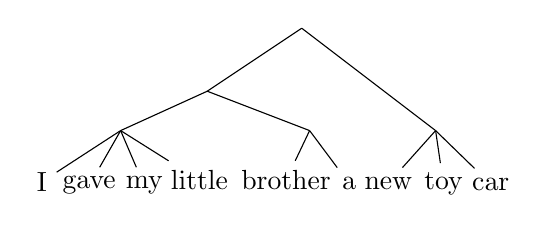
\begin{tikzpicture}
\node (I) at (1,0.05) {I};
\node (gave) at (1.6,0) {gave};
\node (my) at (2.3,0) {my};
\node (little) at (3.0,0.07) {little};
\node (brother) at (4.1,.07) {brother};
\node (a) at (4.9,0.03) {a};
\node (new) at (5.4,0.03) {new};
\node (toy) at (6.1,0.02) {toy};
\node (car) at (6.7,0.02) {car};

\coordinate (Igavemylittle) at (2,0.7);
\coordinate (brothera) at (4.4,0.7);
\coordinate(newtoycar) at (6.0,0.7);
\coordinate (all) at (4.3,2);
\coordinate (Igavemybrothera) at (3.1, 1.2);

\foreach \from/\to in {Igavemylittle/I, Igavemylittle/gave, Igavemylittle/my, Igavemylittle/little, a/brothera, brother/brothera, newtoycar/new, newtoycar/toy, newtoycar/car, Igavemybrothera/Igavemylittle, Igavemybrothera/brothera, all/newtoycar, all/Igavemybrothera}
	\draw (\from) -- (\to);

\end{tikzpicture}
\caption{possible structure...}\label{fig:struct1}
\end{figure}

Formally, there is no reason to discard this structure, but yet everyone that understands the English language will agree that this section is not constructed this way, as we perceive other parts, such as `my little brother', or `a new toy car'. The structures in Figure \ref{fig:struct2} therefore seem more plausible.

\begin{figure}[!ht]
\centering
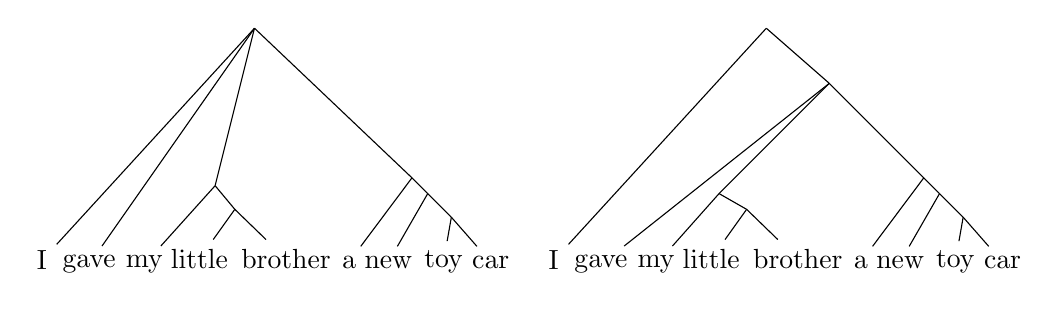
\begin{tikzpicture}

\node (I) at (0,0.05) {I};
\node (gave) at (0.6,0) {gave};
\node (my) at (1.3,0) {my};
\node (little) at (2.0,0.07) {little};
\node (brother) at (3.1,.07) {brother};
\node (a) at (3.9,0.03) {a};
\node (new) at (4.4,0.03) {new};
\node (toy) at (5.1,0.03) {toy};
\node (car) at (5.7,0.03) {car};

\coordinate (toycar) at (5.2,0.6);
\coordinate(newtoycar) at (4.9,0.9);
\coordinate (anewtoycar) at (4.7,1.1);
\coordinate (littlebrother) at (2.45,0.7);
\coordinate (mylittlebrother) at (2.2,1);
\coordinate (all) at (2.7,3);

\foreach \from/\to in {toycar/car, toycar/toy, newtoycar/toycar, newtoycar/new, anewtoycar/newtoycar, anewtoycar/a, littlebrother/brother, littlebrother/little, mylittlebrother/littlebrother, mylittlebrother/my, all/I, all/gave, all/mylittlebrother, all/anewtoycar}
	\draw (\from) -- (\to);

\node (I_) at (6.5,0.05) {I};
\node (gave_) at (7.1,0) {gave};
\node (my_) at (7.8,0) {my};
\node (little_) at (8.5,0.07) {little};
\node (brother_) at (9.6,.07) {brother};
\node (a_) at (10.4,0.03) {a};
\node (new_) at (10.9,0.03) {new};
\node (toy_) at (11.6,0.03) {toy};
\node (car_) at (12.2,0.03) {car};

\coordinate (toycar_) at (11.7,0.6);
\coordinate(newtoycar_) at (11.4,0.9);
\coordinate (anewtoycar_) at (11.2,1.1);
\coordinate (littlebrother_) at (8.95,0.7);
\coordinate (mylittlebrother_) at (8.6,0.9);
\coordinate (gavetobrother_) at (8.1,1.3);
\coordinate (gavetocar_) at (10,2.3);
\coordinate (all_) at (9.2,3);

\foreach \from/\to in {toycar_/car_, toycar_/toy_, newtoycar_/toycar_, newtoycar_/new_, anewtoycar_/newtoycar_, anewtoycar_/a_, littlebrother_/brother_, littlebrother_/little_, mylittlebrother_/littlebrother_, mylittlebrother_/my_, all_/I_, gavetocar_/gave_, gavetocar_/mylittlebrother_, gavetocar_/anewtoycar_, all_/gavetocar_}
	\draw (\from) -- (\to);
\end{tikzpicture}
\caption{Possible compositional structures for the sentence `I gave my little brother a new toy car'}\label{fig:struct2}
\end{figure}

Such tree representations can be used to capture any compositional structure, although it is often assumed that the nodes (corresponding to the parts) constitute contiguous sequences in the sentence, as such structures can be generated by context-free grammars. Sometimes, this gets in the way, as can be concluded from the tree depicted in Figure \ref{fig:struct3}, where the parts that naturally belong together are found in different places of the sentence.

\begin{figure}[!ht]
\centering
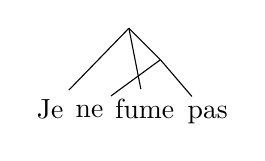
\begin{tikzpicture}

\node (je) at (0,0.07) {Je};
\node (ne) at (0.5,0.04) {ne};
\node (fume) at (1.2,0.08) {fume};
\node (pas) at (2,0) {pas};

\coordinate (nepas) at (1.4,0.7);
\coordinate (jefume) at (0.6,0.7);
\coordinate (all) at (1.0,1.1);

\draw (nepas) -- (ne);
\draw (nepas) -- (pas);
\draw (je) -- (all);
\draw (fume) -- (all);
\draw (all) -- (nepas);

\end{tikzpicture}
\caption{'non-projective' tree}\label{fig:struct3}
\end{figure}

Of course it is practically impossible to automatically assign structures to sentences without labelling the nodes of such structures. Say something about standard ways to do this? Say why it is not relevant for this thesis
+ not way to know if it is consistent without labelling!!!


\section{Translation Structures}

Even when assuming compositional grammars for two languages exist, it is still questionable whether it is possible to find a mapping between the two grammars. Of course, in theory we could just create a mapping that maps entire source structures to entire target structures, in practice, however, we cannot.\footnote{An besides, but if this were possible, we might as well just create a mapping that maps entire source sentences to entire target sentences and be done with it.} A mapping should thus map parts of structures to parts of structures, and combine these parts into a new structure (thus in a compositional way). Once again, we start with a theoretical discussion of mappings, followed by a discussion of how ..... in practice.
 
\subsection{Theory}

As compositionality of language, compositionality of translation is described in a principle:

\begin{quote}
\textbf{The Principle of Compositionality of Translation}\\
Two expressions are each others translation if they are built up from parts which are each other's translation, by means of translation-equivalent rules (ref??)
\end{quote}

In other words, compositional translation takes place by identifying the compositional structure of the target language, mapping the syntactic rules to translation equivalent rules on the source side, and recursively determining the translation equivalence of the parts. Compositional translation is a very common method in translation between artificial languages \citep{janssen1996compositionality,janssen1998algebraic}. The translation from one logical language into another, or the translation the compiler performs when interpreting a programming language are all compositional. When considering a purely semantical compositional grammar, it seems that compositionallity of translation should also hold for natural language, yet it is unclear if translation can actually be executed this way. We will discuss the main issues.

An important assumption that is underpinning the principle, is that in translation not only meaning, but also form should be preserved (as much as possible. In other words, it assumes that translation is literal. For artificial languages this property is straight-forward and useful, mostly because there are no a priori reasons to prefer a non-literal translation over a literal translation. In natural language, this assumption is more questionable. There are many occasions in natural language in which similar arguments apply. It captures, for instance, the fact that `all ravens are black' is an adequate translation of `alle raven zijn zwart', while the logical equivalent `if something is not black it is not a raven' is not \citep{landsbergen1989power}. However, in practice a translator can have many reasons to prefer a free translation even if a more literal alternative is also available. In MT-systems, this issue is often ignored, which does not seem like a huge concession, given that the these systems are not (yet) focussing on literary translations, and the most literal translation is often a good, or at least an acceptable translation.

A second problem with compositional translation are translational divergences (anders?), syntactic or even lexical. Languages do not always express the same set of meanings in the same way. Even in languages of cultures that are quite similar, one can find a number of words that simply do not have an adequate translation in the other language (e.g., in translation between English and Dutch the words `gezellig' and `evidence' do not seem to have a clear equivalent in the other language), and even if the same meaning is expressed there are many syntactic phenomena in natural language that seem to be problematic for a compositional translation.  For example: different ways of role expression (e.g., `I like ...' and `\textcyr{mne nravitsa ...}') or syntactic mismatches (e.g., `woonachtig zijn' and its translation `reside' \citep{landsbergen1989power}).  (anders) The grammars rules and basic units can thus not simply be taken from a monolingual grammar, as there is no guarantee that the rules and basic units will have a translation equivalent rule or basic unit in the other grammar. The grammars must be constructed for translation, such that they are `attuned' \citep{rosetta1994compositional}, which is a non-trivial task. \cite{rosetta1994compositional} showed that previous mentioned examples do not necessarily stand in the way of compositional translation, by manually constructing a grammar for translation from English to Dutch, covering many non-trivial translation phenomena. However, their grammar consist of separate semantic and syntactic formalisms, which makes their case more complicated than the more direct structure mapping we are interested in for this thesis.

In summary, even when the existence of compositional structures for languages and literalness of translation is assumed, there is no guarantee that the structures of the two languages can be linked in a consistent fashion. Suitable compositional structures for a language might thus depend on which language it should be translated in. The nature of this problem suggests that if compositional syntactic structures for languages  can be constructed, they should have a strong semantic motivation.

\subsection{In Practice}

Compositional structures of translation are representation-wise very similar to compositional structures of language: they are tree representations that describe how the sentence was compositionally translated. The difference lies in the notion of parts: in compositional language structures, the parts were sequences of words that were combined through syntactic relations, while in compositional translation structures, the parts are defined through translation equivalence. Consider, for instance, the sentence pair (I give my little brother a ball, Ik geef mijn kleine broertje een bal), in which the translation equivalence is made explicit through linking the `parts' that were used in the translation. Note that if tree pairs are constructed as such through compositionality, every source node tree has an equivalent target node tree, the two resulting trees are thus isomorphic.

\begin{figure}[!ht]
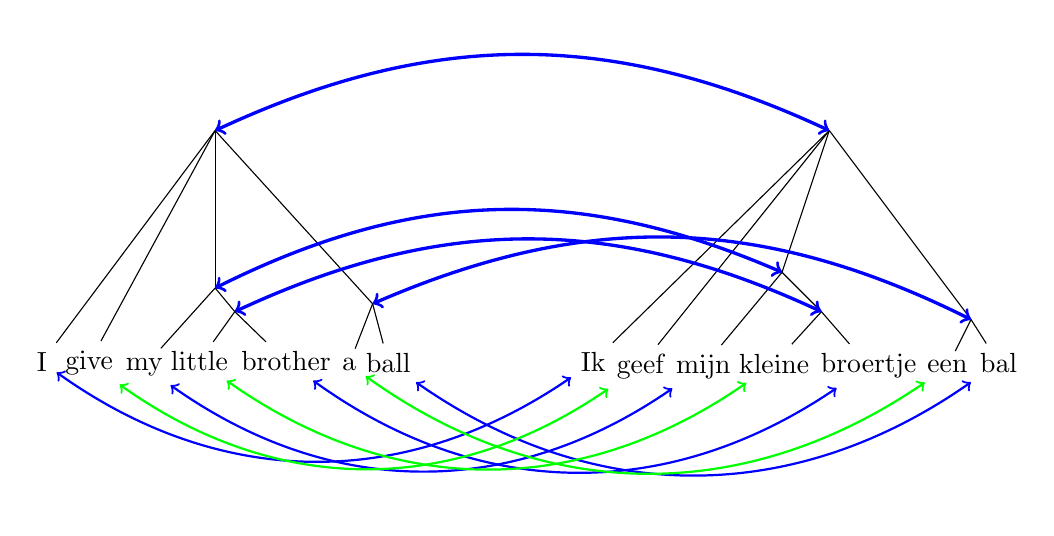
\begin{tikzpicture}

\node (I) at (1,0.06) {I};
\node (give) at (1.6,0.05) {give};
\node (my) at (2.3,0) {my};
\node (little) at (3.0,0.07) {little};
\node (brother) at (4.1,0.07) {brother};
\node (a) at (4.9,0.03) {a};
\node (ball) at (5.4,0.05) {ball};

\coordinate (toycar) at (5.6,0.7);
\coordinate (littlebrother) at (3.45,0.7);
\coordinate (mylittlebrother) at (3.2,1);
\coordinate (aball) at (5.2,0.8);
\coordinate (all) at (3.2,3);

\foreach \from/\to in {aball/ball, aball/a, littlebrother/little, littlebrother/brother, mylittlebrother/my, mylittlebrother/littlebrother, all/give, all/mylittlebrother, all/aball, all/I}
	\draw (\from) -- (\to);
	
\node (Ik) at (8,0.06) {Ik};
\node (geef) at (8.6,0) {geef};
\node (mijn) at (9.4,0) {mijn};
\node (kleine) at (10.3,0.04) {kleine};
\node (broertje) at (11.5,0.01) {broertje};
\node (een) at (12.5,0) {een};
\node (auto) at (13.15,0.05) {bal};

\coordinate (kleinebroertje) at (10.9,0.7);
\coordinate (mijnkleinebroertje) at (10.4,1.2);
\coordinate (eenauto) at (12.8,0.6);
\coordinate (alles) at (11,3);

\foreach \from/\to in {eenauto/auto, eenauto/een, kleinebroertje/kleine, kleinebroertje/broertje, mijnkleinebroertje/mijn, mijnkleinebroertje/kleinebroertje, alles/Ik, alles/geef, alles/mijnkleinebroertje, alles/eenauto}
	\draw (\from) -- (\to);	

\foreach \from/\to in {all/alles, mylittlebrother/mijnkleinebroertje, littlebrother/kleinebroertje, aball/eenauto}
	\draw[<->, bend left =25, very thick,blue] (\from) to (\to);

\foreach \from/\to in { broertje/brother,  mijn/my, Ik/I, auto/ball}
	\draw[<->, bend left =35, thick,blue] (\from) to (\to);

\foreach \from/\to in {een/a,  kleine/little, geef/give}
	\draw[<->, bend left =35, thick,green] (\from) to (\to);

\end{tikzpicture}

\caption{linked structures}\label{fig:transtrees}
\end{figure}

Unfortunately, the simplicity of the given example is far below average: there is no translational divergence (in fact, the target sentence is a word for word translation of the source sentence, and could be compositionally translated through any possible structure, as all contiguous sequences of words have a translation equivalence in the other sentence), establishing the translation equivalent parts is really easy (anders), and the sentences have the same length.






We have already mentioned, that monolingually motivated compositional structures are not necessarily suitable for translation. We have now arrived at a new situation:

\begin{figure}
\centering
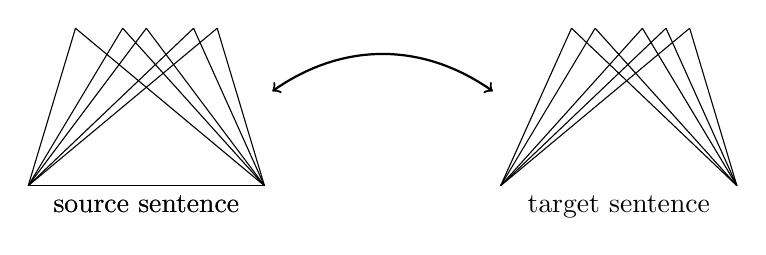
\begin{tikzpicture}

\coordinate (ss) at (1.5,0);
\node [below] at (ss) {source sentence};

\draw[] (0,0) -- node[below]{source sentence} (3,0);
\draw (0,0) -- (0.6,2) (3,0) -- (0.6,2);
%\draw (0,0) -- (0.9,2) (3,0) -- (0.9,2);
\draw (0,0) -- (1.2,2) (3,0) -- (1.2,2);
\draw (0,0) -- (1.5,2) (3,0) -- (1.5,2);
%\draw (0,0) -- (1.8,2) (3,0) -- (1.8,2);
\draw (0,0) -- (2.1,2) (3,0) -- (2.1,2);
\draw (0,0) -- (2.4,2) (3,0) -- (2.4,2);

\coordinate (ts) at (7.5,0);
\node [below] at (ts) {target sentence};

%\draw (6,0) -- (0.6,2) (9,0) -- (6.6,2);
\draw (6,0) -- (6.9,2) (9,0) -- (6.9,2);
\draw (6,0) -- (7.2,2) (9,0) -- (7.2,2);
%\draw (6,0) -- (7.5,2) (9,0) -- (7.5,2);
\draw (6,0) -- (7.8,2) (9,0) -- (7.8,2);
\draw (6,0) -- (8.1,2) (9,0) -- (8.1,2);
\draw (6,0) -- (8.4,2) (9,0) -- (8.4,2);

\coordinate (startarrow) at (3.1,1.2);
\coordinate (endarrow) at (5.9,1.2);

\draw[<->,bend left =35, thick] (startarrow) to (endarrow);

\end{tikzpicture}
\caption{matching compositionality of translation and compositionality of natural language.}\ref{fig:comp2x}
\end{figure}
explain how parts should be nodes..

Explain how we assume that the notion of parts is the same as before: nodes. once again we begin by not assuming label?
 thus every node should have an equivalent in the translation structure on the other side (thus bijective mapping between non-terminal nodes). A very straight forward example is given in Figure 

In some cases, this is very straight forward:



Trees that can be linked this way can be generated by SCFG's that have only terminals or only non-terminals at the right hand-side, respectively. It may now be easier to see why such a grammar without any labels is not particularly informative. The grammar generating this particular tree, would be:

\begin{figure}[!ht]
\begin{tabular}{lll}
X $\rightarrow$ $\langle$ X$_1$ X$_2$ X$_3$ X$_4$, X$_1$ X$_2$ X$_3$ X$_4$  $\rangle$ && X $\rightarrow$ $\langle$ give, geef $\rangle$\\
X $\rightarrow$ $\langle$ X$_1$ X$_2$, X$_1$ X$_2$ $\rangle$ && X $\rightarrow$ $\langle$ I, ik $\rangle$ \\
X $\rightarrow$ $\langle$ my, mijn $\rangle$ && X $\rightarrow$ $\langle$  little, small $\rangle$ \\
X $\rightarrow$ $\langle$ brother, broertje $\rangle$ && X $\rightarrow$ $\langle$ a, een $\rangle$
X $\rightarrow$ $\langle$ ball, bal $\rangle$\\
\end{tabular}
\end{figure}

Which gives generates more 

\section{Empirically studying compositional translation}

Thus far, we have seen that compositional translation knows many difficulties: finding appropriate grammars for both source and target language, disambiguating sentences, and transforming source side structures into target side structures through a mapping. Given the size and nature of natural language, it is impossible to give an indisputable proof of their existence, after all, how can one possibly show that a grammar covers all expressions that can be uttered by a human being. The theoretical question, however, evokes other questions of more practical nature, such as

\begin{itemize}
\item How well are corpora covered by certain grammars?
\item Do monolingual syntactic structures correspond with translation data?
\item What transformational formalism is powerful enough to transform source side trees to target side trees?
\item Can we find methods to systematically assign dual structures to sentences that are each others translation?
\end{itemize}

The availability of huge corpora with pairs of sentences that are each others translation allows for an empirical search to the answer of these questions. This section is meant to make the reader familiar with empirical research related to transfer models. We will identify the assumptions made to make such analyses possible, and explicate a few concrete questions that can be asked given this starting point. In the subsequent section, we will explicate a few concrete questions that can be asked given this starting point, and discuss the answers empirical research conducted prior to this thesis resulted in.


\subsection{Correctness of the Translation Data}

As mentioned before, empirical analyses are based on parallel corpora with texts that are each others translation. These texts were not primarily created to provide data for MT, and might thus also not be perfectly suitable for that. To train MT models, infrequent mistakes in the data are generally not problematic, as they will receive a low probability. This is not the case for empirical analysis. Nevertheless, there seems to be no other option than to assume the corpus is perfect for this purpose. We will discuss three assumptions made about the data.

\myparagraph{1. Corpora are correctly aligned at the sentence level.}
Aligning corpora on the sentence level is not as simple as it might seem. Texts are not always translated sentence by sentence. Short sentences may be merged or long ones broken up, and in some languages there are not even clear sentence delimiters \citep[p.55]{koehn2008statistical}. However, the techniques for sentence alignment are very good (ref??), it thus seems very reasonable to assume that the aligned sentences in the corpora do in fact have the same meaning.

\myparagraph{2. The translations in the corpora are correct}
The texts are produced by humans, who sometimes make mistakes. To use the corpora, we have to assume that the aligned sentences are good translations of each other. Ref about quality??

\myparagraph{3. Translation is literal.}
 One English sentence often has many translations in another language, as similar meanings can be expressed in multiple ways. For instance `jeg giver dig blomster' is a good Danish translation of `I give you flowers', but so it `jeg giver blomster til dig' (and these translations are actually even rather close). Especially when one text is not a direct translation of the other text, but the two are for instance just separate reports of the same event, it might happen that sentences do have the same meaning, but are not very similar in form. In empirical analyses it is assumed that at least the vast majority of the translations in the corpora are rather literal.

\subsection{Word Alignments}

To study the structure of translation, we need alignment on an even granularity. Virtually all empirical analyses of translation data are based on word-alignments, i.e. mappings from source to target words that describes which target words were involved in the translation of which source words. As word-alignment are the only mainstay in how the sentence was translated, they are of crucial important for a deeper analysis of translation structures. The current techniques for word-aligning corpora are not as good as the techniques for sentence alignments. For empirical analysis often one of the few manually aligned corpora is used. A formal definition of word-alignments, some information of the forms they occur in, and a description of the issues with generating them, can be found in Section \ref{sec:alignments}.

\subsection{Syntactic Parsers}

The third main assumption made in empirical analyses is not directly related to translation, but to other area's of natural language processing. To analyse translation data is often made use of parsers to generate monolingual syntactic structures for one or both sides of the corpus. 


\section{Empirical Analyses}

After having expounded the main assumptions of empirical research of translations, we can get to the concrete questions asked in such research. Recall that theoretically we are interested in the possibility of finding structures for source and target structures and mappings between them. There are several questions that might be answered by empirical research that closely relate to this theoretical question, that can be divided into more linguistically and more formally oriented questions, such as:

such as\begin{enumerate}
\item How well do monolingual syntactic constituents cohere across languages?
\item What is the minimum rule depth we need to find correspondences for entire syntactic source and target trees of a sentence pair?
\item What is the minimum rank of a formal SCFG that can cover the entire corpus?
\item What part of a corpus can be covered by a binary SCFG?
\end{enumerate}


\subsection{Linguistic Trees}

Several studies focus on the explanatory power of transforming linguistic parse trees, thus addressing the first two questions. Even though they are ran on different datasets, with different language pairs and use different criteria, they all find that linguistic parse trees do not coincide very well with translation corpora.

\subsubsection{Constituency grammars}

There are different ways of quantifying the suitability of monolingual linguistic parse trees. An often cited study is the one carried out in \cite{fox2002phrasal}. \citeauthor{fox2002phrasal} investigated how well linguistic phrases (i.e., constituents in a parse tree) stay preserved during translation from English to French. For her investigation, she used a manually aligned corpus created by \cite{och2000improved}, which contains 500 randomly selected sentences from the Canadian Hansard corpus. The manual alignments in this corpus are of type `sure' ($S$) and `possible' ($P$).\footnote{A more detailed description of the difference between these two alignment links can be found in Section \ref{sec:alignments}}. Fox counted the number of times the translation of distinct syntactic constituents (on the English side) overlapped or `crossed' (we will not five a formal definition of a `crossing', but provide an example in Figure \ref{fig:fox}. She concluded that crossings - even after filtering out phrasal translations that necessarily result in crossings - are too prevalent to ignore (on average 2.854 per sentence if all alignment links are considered).\footnote{With a manual analysis of the crossings in the constituency parses she showed that many of them are not due to the lac of phrasal cohesion, but are caused by errors in the syntactic analysis or rewording and reordering in the translation. Her analysis, however, included only the crossings of the S aligment links - the ones on which all annotators agreed and that were not ambiguous - that constitute just a small part of the total set of crossings.}


\begin{figure}[!ht]
\centering
\includegraphics[scale=0.4]{crossing.png}
\caption{An example of a crossing according to \cite{fox2002phrasal}. Further explain.}\label{fig:fox}
\end{figure}

Her results are supported by others. \cite{galley2004s} focussed on the second question posed on the beginning of this Section. They generated constituency trees on the English side of the aforementioned Hansard corpus and tested how powerful a synchronous grammar should be to be consistent with the translation corpus. The power of the grammar was expressed in terms of the depth of the subtrees it generated, a standard CFG rule, that generates only single non-terminals, thus has depth 1. If rules of larger depth than 1 are needed, the non-terminal nodes of the syntactic source tree cannot be mapped bijectively to any target tree in a way consistent with the word-alignments. He found that only 19.4\% of the trees in the corpus could be entirely covered by one-depth-rules, and 85\% of the nodes (for the S alignments). Furthermore, he found that to cover the entire corpus with a grammar consistent with the allowed number of rule expansions should be no less than 17 for the S-alignments, and 23 for automatic alignments. For the English-Chinese corpus he analysed (FIBS, reference??), the coverage of low-expansion rules was even lower: 16.5\% (of the trees) for rules with a single expansion, and 100\% only with a maximum of 43\% expansions per rule.

\cite{khalilov2012statistical} confirmed the inadequacy of child-reordering in work that focusses on source reordering preliminary to translation. Using LRscore \citep{birch2010lrscore} as a measure of success, they concluded that permuting the children of nodes in a constituency tree is insufficient to reach a perfect permutation of source-words in English-Dutch and English-Spanish translation data, even when deleting up to 5 layers of nodes in the parse tree is allowed.\footnote{Their score for English-Spanish, however, is surprisingly high: around 94.}


\subsubsection{Dependency Grammars}

Not very much literature focusses on the consistency of dependency grammars with translation data, but some articles can be found on the matter. In her study about crossings, \citeauthor{fox2002phrasal} also devoted a section on dependency grammars. She observed that dependency parses are more cohesive than constituency grammars, with
2.714 crossings per sentence, compared to 2.854 for constituency grammars. A study that exclusively focusses on dependency parses was presented in \cite{hwa2002evaluating}. She investigated how well predicate argument structures agree between English and Chinese, addressing the validity of the Direct Correspondence Assumption.\footnote{Which expresses the intuition that there exists a mapping between the syntactic relationships in two sentences that are each others translation, and is thus directly allied to compositional translation} \citeauthor{hwa2002evaluating} evaluated the quality of Chinese dependency parses that were projected directly from English to Chinese through a manual word-alignment. The resulting parses ha a very low F-score (38.1), which is not surprising, as phrasal translations (multiple aligned words on source or target side) and unaligned target words always result in errors. \citeauthor{hwa2002evaluating} also observed this fact. They developed a small set of linguistically motivated rules, which boosted the F-score to 68.3, which is significantly higher, but still rather low. Also, it makes their work very specific, and hard to extend to other language pairs or contexts.

Another work along the same lines was presented by \cite{fung2006automatic}. \citeauthor{fung2006automatic} did not directly use dependency grammars, but learned cross-linguistic (English-Chinese) semantic verb frames. The learned argument mappings  had an accuracy of 89.3\%. It is unclear how their results compare to \citepos{hwa2002evaluating} results and dependency grammars in general, a fortiori because the exact nature of the learned semantic frames stays unclear.

\subsection{Formal Trees}

A second line of empirical research does not restrict source (or target) side trees to linguistic trees, but investigates the coverage of formal SCFG's. The majority of the empirical results on SCFG's focus on the coverage of binary trees \citep[e.g.,]{zhang2006synchronous,huang2009binarization}, or SCFG's in normal form \citep[e.g.,][]{sogaard2009empirical1,sogaard2009empirical2,sogaard2010can}. All concluded that the range of reordering phenomena occurring in real translation data are by far not as complicated as the worst case scenario sketched in \cite{satta2005some}.
%But also that...?

\cite{wellington2006empirical} seem to be the only one who compared their results with linguistically restricted parse trees. On several dataset (covering translation from Chinese, Romanian, Hindi, Spanish and French to English), he found that maximally 5\% of the alignments could not be explained by a completely binary tree, while the failure rate for binary trees that were constrained by monolingual parse trees on the English side climbed to 15\% for French/English to 61\% for Chinese/English. The failure rate they found for non constrained binary trees is much lower than the one found by \cite{simaan2013hats}, who reported a coverage of 71.46\% for the manual alignments of the Hansard corpus for trees with a maximal branching factor of 2. The coverage of binary trees for automatic alignments was even lower: 52.84\%. This difference between the results of \cite{wellington2006empirical} and \cite{simaan2013hats} is most likely due to a different treatment of alignment links: the latter authors used all alignment links in the dataset, while the former treated many-to-one alignment links disjunctively, focussing on lower bounds. \cite{simaan2013hats} also reported the coverage of non binarisable (permutation) trees, which is surprisingly enough not much higher: 72.14\% and 56.56\% for manual and automatic alignments, respectively.


\chapter{A new analysis???}

It seems that in all these analyses, still no sufficient answer is found to the most general empirical question ....

explain once again contribution this paper?


In this chapter we describe the basis of our investigation, of which some things have already come up in the previous chapters, on a formal level. We will start with a section on alignments, in which we both define these .... blabla. Then, we will describe the set of rules we consider

%Describe it as structures or as rule set.


\section{Alignments}
\label{sec:alignments}

From the previous chapters it has become clear that word-alignments are very important for both MT models and empirical analyses of MT data. In this section, we will provide a more elaborate description of word-alignments than we have before. We will give a definition, discuss the different types of word-alignments and describe the most common method of generating them.

Let us start with an example. Recall that word-alignments are mappings from source to target words that describe how the sentence was word-for-word translated. Alignments can be visualized in many ways, in this thesis, we will visualize alignments using lines or arrows (see Figure \ref{fig:alignment}), in which an arrow from source word $w_s$ to target word $w_t$ thus implies that $w_t$ was involved in the translation of $w_s$. From the sentence in 


\begin{figure}[!ht]
\centering
\includegraphics[scale=0.6]{alignment.png}
\caption{A one-to-one alignment of the Dutch sentence `Na regen komt zonneschijn' and its translation `Auf regen folgt sonneschein'. The alignment visualiser created by \cite{maillette2010visualizing} was used to create this picture.
}\label{fig:alignment}
\end{figure}


\subsection{Formally}

The precise definition of a word-alignment varies from paper to paper. Throughout this thesis we will use the following definition:

\begin{definition}[Alignment]
Given a source sentence $s = s_0 \ldots s_n$ and its translation $t = t_0 \ldots t_m$, an alignment $a \subseteq \{0,1,\ldots,n\} \times \{0,1,\ldots,m\}$ such that $(x,y)\in a$ iff $s_x$ is translated into $t_y$.
\end{definition}

Note that the absence of a $y$ such that $(x,y)\in a$ means that $x$ is unaligned (and the other way around for $y$). In some definitions unaligned words are explicitly included in the alignment by adding an extra $NULL$ token to both source and target sets and including $(x,NULL)$ (or ($(NULL,y)$) in $a$ whenever word $x$ (or $y$) is unaligned.


\subsection{Types of Word-alignments}

In the alignment in Figure \ref{fig:alignment}, every source word is aligned to exactly one target word and vice versa. Such an alignment is called a one-to-one alignment. It is also possible for source and target words to be aligned to more than one word, or to none at all, resulting in alignments that are one-to-many, many-to-one or even many-to-many. Another interesting property of the alignment depicted in Figure \ref{fig:alignment}, is that the target word order is identical to the source word order, resulting in an alignment in which none of the alignment links are crossing. Such an alignment is called monotone. A summary of the restrictions corresponding to these different types of alignments is provided in Table \ref{table:alignments}.

\begin{table}[!ht]
\footnotesize{
\begin{tabular}{|ll|}
\hline
one-to-one & $\forall x\forall y \big( (x,y)\in y \to \forall z \big( (z,y)\in a \to z=x \land (x,z) \in a \to z=y \big ) \big ) $\\
&\\
one-to many & $\forall x\forall y \big( (x,y)\in y \to \forall z \big( (z,y)\in a \to z= x \big) \big) $\\
&\\
many-to-one & $\forall x\forall y \big( (x,y)\in y \to \forall z \big( (x,z)\in a \to z=y \big) \big ) $\\
&\\
many-to-many & - \\
&\\
monotone & $\forall w \forall x\forall y \forall z \big ( \left ( (x,y)\in a \land (w,z)\in a \land x < w \right ) \to y < z \big )$\\
\hline
\end{tabular}
}
\caption{Alignment types, restrictions}
\label{table:alignments}
\end{table}


\subsection{Generating Word-alignments}

Word-alignments are not visible in translation data, and it is not always easy to establish which words should be aligned to which words. We will give two examples to illustrate this.

Obvious examples present itself in the form of idioms (anders). The expression `Every cloud has a silver lining'  is synonymous with `Na regen komt zonneschijn', but it is unclear what would be a good alignment. Arguably, `has' should be aligned with `komt', as they are the only verbs in the sentence pair. However, when asking a bilingual Dutch and English speaker if `has' is a proper translation of `komt', the odds of obtaining a affirmative answer are very slim. A more plausible alignment would be the one that aligns every Dutch word to every English words, indicated that the expression is translated as a whole. Such an alignment is called a phrasal alignment.

Problems also arise in the translation of function words, that do not have a clear translation equivalent in the other language. Consider, for instance, the word `does' in the sentence pair `john does not live here, john wohnt hier nicht'. As `does' has no clear translation in German, one might argue that it should be unaligned. However, the word seems to be connected with `live', so it could also be aligned with `wohnt'. A third option is to align `does' to `nicht', as it appeared with `not' when the sentence was negated.\citep[Example from][p.114]{koehn2008statistical}

\subsubsection{Manual Word-alignments}

In manually aligned corpora, the issues raised in the previous paragraph are often addressed by distinguishing sure alignment links and possible alignment links \citep{lambert2005guidelines}. The sure alignment links (indicated by the letter S) then represent unambiguous alignment links, while the possible alignment links (P) are less certain. Possible alignment links appear in case of phrasal translations, ambiguous translations, or in case two annotators disagree. 

There are very few manually aligned corpora, the only ones known to the author are presented in \cite{och2000improved}, \cite{graca2008building}, \cite{mihalcea2003evaluation} and \cite{pado2006optimal}, \cite{ahrenberg2000evaluation}. Short description of these corpora??
Manually annotating translation corpora is very labour intensive and none of these corpora are big enough to train models in. Rather, they are used to evaluate automatically generated word-alignments. A common metric used for this task is the alignment error rate (AER), that is defined as follows (ref):

$$
\text{AER(S;P;A) = } - \frac{|\text{A}\cap\text{S}| + |\text{A}\cap\text{P}|}{|\text{A}| + |\text{S}|}
$$

A perfect score can thus be achieved by an alignment that has all the sure alignment points and some of the possible alignment points.

\subsubsection{Automatic Word-alignments}

Word alignments are established as a by-product for the word-based IBM models, and despite multiple efforts to improve on these alignments (e.g., refs), it is still common practice to use the alignments produced by the SMT toolkit used to train the IBM models \citep{och03:asc}. We will not discuss further methods for automatically word aligning corpora, but just briefly explain how the IBM alignments arise, and how many-to-many alignments are derived from them.

One step in the IBM models, is to learn a lexical translation model from a parallel corpus. If a word-alignment was directly visible from the data, this would be an easy task, as one could just count for each word how often it occurred in the text and how it was translated, and estimate a probability from these counts using relative frequency estimation (which happens to be the maximum likelihood solution) (anders). Conversely, given the lexical probability model, the most possible word-alignment could be estimated. Learning word-alignments and lexical probabilities from a parallel corpus can thus be seen as a problem of incomplete data, that can be addressed with the expectation maximization (EM) algorithm \citep{dempster1977maximum}, which works as follows:\begin{enumerate}
\item Initialize the lexical probabilities (often with uniform distributions).
\item Compute the most probable alignment from the lexical probabilities (expectation).
\item Recompute the lexical probabilities from the alignment found in the previous step (maximization)
\item Iterate steps 2 and 3 until convergence.
\end{enumerate}

In IBM model 1 and 2, the models that describe how the alignments depend on the lexical probabilities are sufficiently simple to exhaustively run the EM algorithm, and a (global) optimum is thus guaranteed to be found. To find the most probable alignments in the higher IBM models, stochastic hill climbing is used. Excellent examples of how the algorithm works on the IBM models can be found in \cite[p88-113]{koehn2008statistical}.

%Check order
The IBM models consider the sequence of target words as being generated by the source words one by one. Therefore, although source words can be aligned to more target words, every target word is aligned to at most one source word and the resulting alignments are thus many-to-one. However, many-to-many alignments are often desired, as they are very common in practice. Alignments used to train SMT models on are often created by running the IBM models in both directions, and combining the resulting alignments. The three most common methods of merging two alignments $A_1$ and $A_2$ are:\begin{enumerate}
\item Union: $A_1\cup A_2$, containing all links from both alignments. The recall of the union will be high (as it contains many links), but as it contains all faulty alignment links from both alignments too, the precision is often quite low.\footnote{Given a set of desired alignment points $A_{gold}$, recall and precision of an alignment $A$ are defined as follows:\\
$$\text{Recall = }\frac{|A \cap A_{gold}|}{|A_{gold}|} \text{\hspace{10mm}Precision = }\frac{|A \cap A_{gold}|}{|A|}$$
Given the nature of $A_{gold}$, precision and recall are not the common metrics used to evaluate word alignments.}
\item Intersection: $A_1\cap A_2$, containing only the links that occur in both alignments. The resulting alignment is thus a one-to-one alignment. Contrary to the union, the intersection of $A_1$ and $A_2$ (anders) will have a high precision, but a lower recall.
\item A more sophisticated method for combining alignments $A_1$ and $A_2$, is to first take the intersection, ending up with a selection of reliable alignment points, and then extending the alignment by adding neighbouring links as well as links $(i,j)$ for which holds that neither $e_i$ nor $e_j$ was aligned in the intersection \citep{och2000improved}, a heuristic called `grow-diag-final'. Pseudocode of this heuristic can be found in \cite{koehn2008statistical}.
\end{enumerate}

Most current MT models making use of alignments use the grow-diag-final method to obtain their alignments. The resulting alignments have a relatively high precision and recall \citep{och2000improved}, although they still contain several faulty alignment links. As mentioned before, several different alignment models that claim to have better alignment models have been reported (anders). Such methods are often based on .... list some things + references if you come across them. However, none of these methods has really found its way in the MT community. Besides the fact that it is hard to compare alignment methods across domains, it has been shown that improving alignment models does not necessarily result in better MT models... (anders, vind ref, kijk in wu alignment \cite{indurkhya2010handbook}).


\section{Alignment Trees}
\label{sec:alignmenttrees}

Until now, an intuitive understanding of translation structures was sufficient to grasp the questions .... As translation structures are the core topic of .... a more technical discussion is necessary

The core topic of this paper is the structures of translation that, as described in the assumptions of the blabla, are given rise to by alignments. This section, that formally describes these structures, is thus a very important section in this thesis. We will first discuss what a tree-structure is blabla, and how this has manifested itself in MT-models. Then we will discuss the set of structures that is empirically studied in this thesis.

\subsection{Translation Structures from Alignments}



Explain how we see (compositional) translation structures, with an example
%make note about how the examples are very simple

We can describe translation structures with trees, in which the parts are represented by nodes in the tree.

definition of part???






As word-alignments also on larger granularities than words indicate which parts of the target sentence are the translation of which parts of the target sentence, they can be interpreted as instructions of how the translation was built up from its parts. That is, they can be factorized into trees that recursively describe fashions in which the sentence could have been compositionally translated. For whom it is not entirely clear how, an example is included in Figure \ref{fig:atree}.

\begin{figure}
\caption{Example compositional translation tree}\label{fig:atree}
\end{figure}

%Explain relation SCFG's and alignment trees
As the rules of a 
Devising alignment trees is thus closely related to the formally syntactic transfer models described in section \ref{subsec:learningSCFGs}.




In this thesis, we are interested in the constraints an alignment puts on the structure of the source sentence. As this depends solely on the positions the source words were mapped, we will introduce, as far as this thesis goes, a slight change in notation, that better serves this purpose. Following \cite{simaan2013hats}, we will represent an alignment by an ordered sequence of sets, of which the $n$th element specifies to which target word the $n$th source word maps. In case of a one-to-one alignment, this sequence is thus a permutation of the target word-positions, while in more complex alignment some of the target positions may appear multiple times in the sequence, or not at all. We will refer to such a sequence describing an alignment with the term set-permutation, which is formally defined in Definition \ref{def:sperm}. (anders)


\begin{definition}[Set-permutation]\label{def:sperm}
Given a source sentence $s = s_0 \ldots s_n$, its translation $t = t_0 \ldots t_m$, and an alignment $a$, let $a(i) = \{j~|~(i,j)\in a\}$ be the set with target positions that is linked to source position $i$. The set-permutation $\pi$ uniquely describing $a$ is defined as the ordered sequence of sets
$\langle a(0), \ldots, a(n) \rangle$
\end{definition}

%Add example
The set-permutation $\pi=\langle \pi_0,\ldots\pi_n\rangle$ describing the alignment ..... give example for whichever alignment was depicted last. In the coming definitions, we will assume that $\bigcup_{i=0}^{n} \pi_i$ constitutes a contiguous sequence of numbers. In practice, such a situation can always be achieved by only numbering the aligned target positions that are aligned, effectively switching the position numbers to the left whenever an unaligned word is found, and can thus be assumed without lot of generality.


\subsection{Translation Equivalence}

%Eerder leg ergens de link tussen compositional translation and transfer!!!
To build trees that describe how an alignment was built up from his parts, we need to have a notion of translation equivalence, describing which subsequences can be seen as parts. According to the principle of compositionality of translation, these parts should be each others translation, resulting in the following definition (in terms of alignment):

\begin{definition}[Translation Equivalence]
Let $(s,t)$ be a pair of a source and target sentence, let $a$ be an alignment between $t$ and $s$, and $a(x)$ the set of words source word $x$ is aligned to. Two sets of source and target words, referred to with $S = s_1,s_2,\ldots s_k$ and $T = t_1,\ldots,t_k$ are called translation equivalent if and only if $\forall s_i\in S a(s_i)  = x \rightarrow (x = \{\} \lor \forall y \in x \exists t_i\in T x = t_i$
\end{definition}

%Explain how this notion coincides with original phrase pairs blabla, except for contiguousness, explain why we often want contiguousness (continuous non-terminals), but why it is often not a good representation of real language. Also explain that it is often required that there is at least one aligned word on both source and target side (to have some lexical evidence.




\subsection{nodes}






\newpage

\section{Dependency Grammars}
\label{sec:depgram}

This section will provide some information about dependency structures, that we will use as guide in our search for consistency in alignment structures. After a short motivation and background section on dependency grammars, we will give a formal definition and some clarifying examples. Subsequently, we will motivate the suitability of dependency structures for translation. We will end with a short section on the current state of the art dependency parsers.

\subsection{Background and Motivation}

Dependency grammar is a formalism for expressing syntactic structures of sentences. Contrary to traditional phrase structure grammars, that aims to establish relations between constituents of a sentence, a dependency grammar does not divide the sentence in phrases. Rather, it is based on the idea that in a sentence all words but one depend on another word in the sentence, via a(n asymmetric) binary relationship that describes how the former word modifies or complements the latter. For instance, in the sentence `I really like writing my thesis', `my' depends on `thesis', as it complements it, and `really' depends on `like', which it modifies. Words can said to have a valency, depending on how many dependents they need to be saturated (e.g., `like' would have a valency of two 2, as it needs both a subject and an object).

Although traditional dependency grammar (DG) has been used by linguists since the Middle Ages \cite{covington1990dependency}, modern DG is often seen as being created by \cite{tesniere1959elements}, whose cognitive motivation for it is worth citing:

\begin{quote}
The sentence is an organised whole; its constituent parts are the words. Every word that functions as part of a sentence is no longer isolated as in the dictionary: the mind perceives connections between the word and its neighbours; the totality of these connections forms the scaffolding of the sentence. The structural connections establish relations of dependency among the words. Each such connection in principle links a superior term and an inferior term. The superior term receives the name governor; the inferior term receives the name dependent.\footnote{translation: ...}
\end{quote}

The criteria for being a head-dependent pair are a mix of syntactic and semantic criteria \citep{nivre2005dependency}, and generally depend on the grammatical function the sentence or with respect to the word it depends on. Not all dependency grammars are identical in the relations they are considering, and their treatment of certain intuitively problematic constructions as coordination and conjunction \citep{nivre2005dependency}.

\subsection{Formally}

A dependency grammar is a quadruple $\langle R,L,C,F\rangle$, consisting of a set $L$ of terminal symbols (lexemes), a set $C$ of auxiliary symbols (lexical categories), a $R$ set of dependency rules over the auxiliary symbols $C$, and an assignment function $F : L\rightarrow C$.\citep{hays1964dependency,gaifman1965dependency}

A dependency structure of a sentence $s = w_1~\ldots~w_n$ generated by such a grammar can be seen as a directed acyclic graph $\mathcal{G} = \langle V, E\rangle$, in which $V = \{w_1, \ldots,w_n\}$ and $E$ is a set of edges such that $(w_i,w_j)\in E$ if and only if there is a dependency relation between $w_i$ and $w_j$. Furthermore, the graphs satisfies the following two criteria:
\begin{enumerate}
\item $\exists! w\in V \forall w'\in V (w,w')\notin E$ (rootedness)
\item $\forall w_1 w_2 w_3 \in V( (w_1,w_3)\negthinspace\in\negthinspace E \land (w_2,w_3)\negthinspace \in\negthinspace E ) \rightarrow w_1 = w_2$ (single-headedness)
\end{enumerate} 

In other words: a well-formed dependency structure is a tree. The edges of a dependency graph (or branches of the tree) can be labelled with the function of the dependent. An example of such a labelled dependency graph is depicted in Figure \ref{fig:depgraph}.

\begin{figure}
\centering
\begin{dependency}[theme=simple]%[hide label]
\begin{deptext}[column sep=.5cm, row sep=.1ex]
%PRP\$ \& NN \& RB \&[.5cm] VBZ \& VBG \& NN \\
My \& dog \& also \& likes \& eating \& sausage \\
\end{deptext}
\deproot{4}{}
\depedge{2}{1}{poss}
\depedge{4}{2}{nsubj}
\depedge{4}{3}{xvmod}
\depedge{4}{5}{xcomp}
\depedge{5}{6}{dobj}
\end{dependency}
\caption{Dummy Dependency Graph, find other later}\label{fig:depgraph}
\end{figure}

A third criterion that is often used is projectivity, that prescribes a linear ordering of the nodes in the tree. Projectivity simplifies parsing (ref), as it reduces the space of possible dependency parses, but it is often argued that it deprives dependency grammar from its most important asset \citep{covington1990dependency,debusmann2000introduction}: the elegant method for handling discontinuous constituents (see Figure \ref{fig:npdeptree}). For fixed word order languages like English, in which phrases belonging together tend to stay together, projectivity is thus a reasonable criterion, but to account for languages in which there are less restrictions on the word-order (e.g., Russian, Latin) non-projectivity is often required to provide an intuitive analysis. An example of a non-projective in a otherwise fixed word-order language (Dutch) is depicted in Figure \ref{fig:npdeptree}.

\begin{figure}\label{fig:npdeptree}
\centering
\begin{dependency}[theme=simple]%[hide label]
\begin{deptext}[column sep=.5cm, row sep=.1ex]
Ik \& weet \& dat \& hij \& me \& liet \& winnen\\
\tiny{I} \& \tiny{know} \& \tiny{that} \& \tiny{he} \& \tiny{me} \& \tiny{let} \& \tiny{win}\\
\end{deptext}
\deproot{2}{}
\depedge{2}{1}{}
\depedge{2}{6}{}
\depedge{6}{3}{}
\depedge{6}{4}{}
\depedge{6}{7}{}
\depedge{7}{5}{}
\end{dependency}
\caption{Non projective dependency graph. Provide some explanation}
\end{figure}

\subsection{Dependency Grammar and Translation}
\label{sec:deptrans}

We have argued before that dependency grammars can be seen as of both syntactic and semantic nature.
Explain why we want that

As dependency grammars can be seen as of both syntactic and semantic nature, they seem a good candidate formalism to use in translation. Dependency structures are able to account for 

Wat is het punt dat ik hier wil maken? 

Although dependency grammars do not postulate the existence of non-terminal syntactic categories, dependency graphs do give rise to an hierarchical structure that specifies from which smaller parts the sentence was composed. In case of non-projectivity, the constituents in this structure are not necessarily continuous. For instance, the dependency graph depicted in Figure \ref{fig:npdeptree} tells us that `likes' is the head word of the sentence, and that the sentence is composed of 4 parts: the head `likes', its modifier `also', its noun subject whose head is `dog' and the open clausal complement whose head is `eating'. The complement and subject are further divisible in `My' and `dog', and `eating' and `sausage', respectively. As the tree is projective, all constituents are continuous. Also the graph in Figure \ref{fig:depgraph} prescribes an hierarchical structure: it is composed of the subject `I', the headword `know', and the phrase headed by `liet', that is in its turn built up from its head `liet', `dat', `hij' and the discontinous phrase `me winnen'. Such an hierarchical can not be captured by a phrase structure grammar






As dependency grammars can be seen as of both syntactic and semantic nature, they seem a good candidate formalism to use in translation. Furthermore, if projectivity is not required, is is independent of word order, which addresses on of the major issues of MT. (anders). E.g., all permutations of \textcyr{devuxka vidit mal\char126 qika} are reasonable translations of `The girl sees the boy', which might be hard to capture with a constituency grammar, but is trivial if the dependency structure is considered.


\subsection{Parsing with Dependency Grammars}

section on parsing





different criteria, different models (treating different `hard' cases differently)


\bibliography{thesisDH}
\end{document}